\documentclass[11pt]{article}

\usepackage{fullpage}
\usepackage{graphicx}
\usepackage{hyperref}

\title{GAS SENSOR IN EMERGENCY BROADCAST SYSTEM}
\author{M.Krishnaraj}
\date{\today}

\begin{document}

\maketitle

\section{INTRODUCTION}

In the last decade, various advances have been made in the area of control and industrial automation.From this emerges the Internet of Things (IoT) is the inter-networking of physical devices, vehicles , buildings, and other items embedded with electronics, software and network connectivity that enable these objects to collect and exchange data. Several communication systems are used for fast, efficient and efficient delivery of alerts. Especially for delivering emergency alerts using the broadcasting system, as they are robust to the destruction of the network infrastructure. However, for the flexible broadcasting system, mobility has also been added to the digital broadcasting system. In the automatic emergency alert services (AEAS) standard, this  Terrestrial Digital Multimedia Broadcasting (TDMB) control channel is like an alert service channel. A TDMB control information limits the use of AEAS. When the AEAS is used, while the TDMB channel is very busy with the other TDMB control data. If the receiver is deactivated in the mobile station (MS), the TDMB receiver does not have the functionality to receive the AEAS message. In addition, an activation method for the TDMB receiver disabled in emergencies is required in each system, but in this system, AEAS messages are also delivered to all MS users. The Emergency Signaling Warning System (ESWS), the conventional AEAS system, is described. Deficiencies are compensated. Even if the conventional TDMB channel is very congested, the AEAS allow the effective and fast delivery of emergency alert messages. The performance of the receiver is improved because the periodic feature allows for a more sophisticated channel estimation method. However, to avoid the involvement of channel repeaters used in TDMB systems, AEAS is implemented in the repeater. Users of the repeater service area, such implementation, are inherently efficient location based services (LBS). This allowed the system to avoid consumption of LBS in the mobile
system.

\section{CONFIGURATION OF TDMB}

\subsection{Emergency broadcasting system}

The TDMB EBS can transmit too many emergency alert contents to the environment without relying on any additional receiver operation [14]. The Emergency Broadcast System , sometimes called the Emergency Action Notification System , is a former emergency warning system used in the United States. In the general environment, the system can provide a system repeat service in which the TDMB for the system made in a part of the repeater channel and part of EBS. The radio frequency signal is converted to intermediate frequency signal after filtering and the low noise amplifier. This bandwidth is converted into an IF signal by an IF digital converter and an analog converter is implemented after cancellation and interference equalization. A general repeated TDMB signal and an emergency broadcast signal and the selected signal signal executed by the "Switch" block operates. The switch selects the general IF TDMB sign and transmits the signal to the RF converter in a common environment.

\begin{figure}[h]
\begin{center}
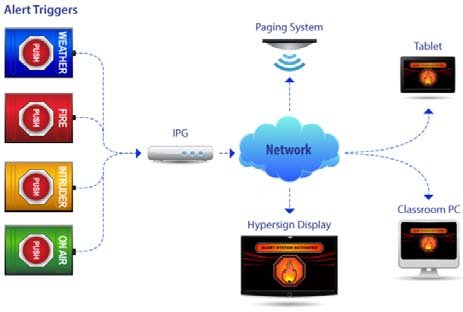
\includegraphics[scale=0.5]{ebs structure.png}
\end{center}
\caption{Diagram of the emergency broadcasting system.}
\label{setup}
\end{figure}

\section{IEEE802.11AH PROTOCOL}

The service related to IoT has an intelligent network scenario based on IEEE802.11AH and backhaul network. The device serves to improve the efficiency, reliability and sustainability of the Smart grid system services. The wireless smart metering service network belongs to the WPAN system. To manage and control the boot data, the Wi-SUN home is attached via the IEEE802.15. The difference between the smart meter and WPAN is 15. 11ah AP is data converted by GW retransmissions over the WiFi protocol IEEE802. The distance between the GW household smart meters is comparatively shorter than the distance between AP and GW. According to the utility database, a decision for the optimal use of utility data is determined by the control and the database, and transmits the domestic intelligent decision command meter through the network of Backhaul and the IEEE802. 11a protocol. The conventional transceiver architecture for IEEE802. 1ah under modulation and coding scheme1, BCC and 2 MHz of bandwidth. The transmitter of the BCC Interleave coding system between RF.

This data format in the OFDM file for the Wi-Fi protocol at 2 MHz bandwidth. With the aim of fully supporting the mobile terminals with the range of repeater service. Wi-Fi is a trademark of the Wi-Fi Alliance, the commercial organization that adopts, tests, and certifies that the devices meet 802.11 standards related
to wireless local area networks. The IEEE 802.11b, IEEE 802.11g and IEEE 802.11n standards enjoy international acceptance because the 2.4 GHz band is almost universally available. Its range is somewhat lower than that of standards working at 2.4 GHz, because the frequency is higher.

\subsection{SENSOR MQ4}

This is a sensor to detect methane gas (gas) in the air; the MQ-4 can detect concentrations of 300 to 10000 ppm. This transducer contains high sensitivity and fast response time. The output has an analogy resistance, it is the sign that allows us to analyse the behaviour. The sensor output is an analogy resistor. The interface circuit is very simple, everything to do with 5V power supply, add a load resistor and connect the output to the analog - digital converter. 

\subsection{ADJUSTMENT OF SENSITIVITY}

The resistance value of MQ-4 is different from several gas concentrations. Therefore, sensitivity adjustment is very necessary. We recommend calibrating the detector for 5000ppm of CH4 concentration in air and using the load resistance value of approximately 20K. When measured with accuracy, the convenient alarm point for the gas detector must be determined after consideration of temperature and humidity

\begin{figure}[!htb]
    \centering
    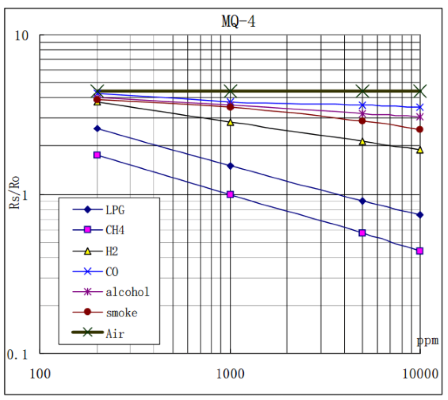
\includegraphics[width=0.8\textwidth]{sensitivity char.png}
    \caption{Shows the typical sensitivity characteristics of
the MQ-4 for several gases.}
    \label{left}
\end{figure} 

\section{PROPOSED SYSTEM}

Several sensors are used in this system. There are three modules; The first module is the design of a web page using the software Dream Viewer and Xampp. Developer to create a web server for testing purposes is a simple and light distribution of Apache , My SQL , Php and PERL. The microprocessor ATMega328p, together with the ESP8266 wifi model and the MQ4 sensor were used to implement the gas sensor. We can observe the programming developed to be able to carry out the acquisition of the data through the sensor using the proposed microcontroller. A program was developed in Labview to observe the measurements made by the MQ-4 sensor.

\begin{figure}[!htb]
    \centering
    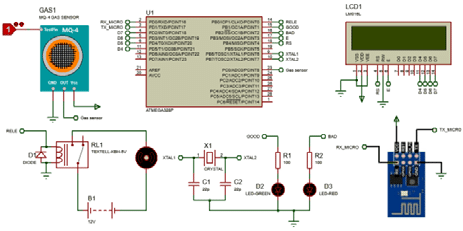
\includegraphics[width=0.8\textwidth]{circuit MQ-4.png}
    \caption{ Circuit implemented for the MQ-4 gas sensor of
the proposed system.}
    \label{left}
\end{figure} 

Free and open source it consists of Apache Http and severe interpreters for scripts written in PHP and PERL Web programming languages and applications using the web page only the user can access the system, to turn on/off the light, the fan and the Gas leak the second module will be the piece of hardware, sensors such as MQ4 gas sensor, IR sensor and MP Proteus software lab to install the third module will be the combination of hardware and software using built-in PHP and C. The WiFi protocol IEEE802.11ah, for long range communication.

\begin{figure}
    \centering
    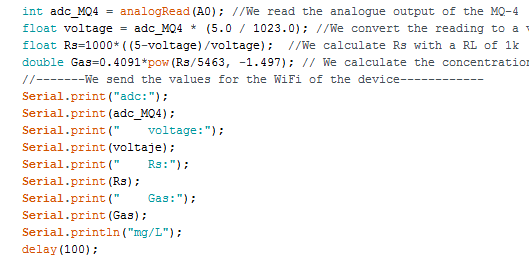
\includegraphics[width=0.8\textwidth]{Aurdino code.png}
    \caption{ Arduino programming for the implementation
of the MQ-4 system sensor.}
    \label{left}
\end{figure}

\newpage

\section{CONCLUSIONS}

This document includes security sensor and infrared, Wi-Fi module, gas sensor for the emergency environment. This document describes the long-range IoT communications based on the IEEE802.11ah Wi-Fi protocol. In which it uses Wi-Fi to send data over the Internet. In the IoT device all the data has been stored and the monitoring has been done through the server. When the device is turned on, the Wi-Fi is automatically connected through the Internet and the data has been shared. This project is designed with the hope that the sea is very economical and useful for the purpose of safety and offering flexibility in operation.

\end{document}

